
We consider the one-dimensional heat equation with Dirichlet, Neumann, and periodic boundary conditions, discretized on a two-qubit register. Unless otherwise stated, the numerical target is the exact discretized solution vector $u(T)=e^{-AT}u(0)$ at total evolution time $T=1$, with oscillator truncation $n_{\mathrm{fock}}=64$ and first-order Trotterization using $n_{\mathrm{trotter}}=100$ steps.

For the numerical study we fix a four-dimensional semidiscrete system encoded on a two-qubit register, with $M=4$, $\alpha=1$, $h=1$, $T=1$, and initial state $u(0)=\ket{01}$. Since $\alpha/h^2=1$ in all three cases, the exact semidiscrete generators used in the simulations are
{\small
\[
\begin{aligned}
A^{(\mathrm D)}&=
\begin{bmatrix}
2&-1&0&0\\
-1&2&-1&0\\
0&-1&2&-1\\
0&0&-1&2
\end{bmatrix},
&&u(0,t)=u(\mathcal L,t)=0,\\[0.5em]
A^{(\mathrm N)}&=
\begin{bmatrix}
1&-1&0&0\\
-1&2&-1&0\\
0&-1&2&-1\\
0&0&-1&1
\end{bmatrix},
&&\partial_x u(0,t)=\partial_x u(\mathcal L,t)=0,\\[0.5em]
A^{(\mathrm P)}&=
\begin{bmatrix}
2&-1&0&-1\\
-1&2&-1&0\\
0&-1&2&-1\\
-1&0&-1&2
\end{bmatrix},
&&u(0,t)=u(\mathcal L,t),\ \partial_x u(0,t)=\partial_x u(\mathcal L,t).
\end{aligned}
\]
}

For normalized states, fidelities are reported as
\[
F(\psi,\phi)=|\langle \psi \mid \phi\rangle|^2
\]
and the exact semidiscrete target is
\[
u_{\mathrm{exact}}(T)=e^{-AT}u(0).
\]
We use
\[
F_{\mathrm{exact}}=F(u_{\mathrm{alg}},u_{\mathrm{exact}}),\qquad
F_{\mathrm{trunc}}=F(u_{\mathrm{alg}},u_{\mathrm{trunc}}),\qquad
F_{\mathrm{oracle}}=F(\psi_{\mathrm{prep}},\psi_{\mathrm{target}}),
\]
where $u_{\mathrm{trunc}}$ is the exact finite-Fock reference induced by the same kernel parameters and $\psi_{\mathrm{target}}$ is the ideal truncated oscillator state. The quantities $F_{\mathrm{snap}}$ and $F_{\mathrm{givens}}$ denote the end-to-end PDE fidelities obtained with SNAP$+$D and Givens preparation, respectively. The CV postselection probability is
\[
p_{\mathrm{post}}
 :=
\left\|
(\langle 0|\,S^\dagger(r_{\mathrm{target}})\otimes I)\,\Psi_{\mathrm{out}}
\right\|^2 .
\]
The quantity $n_{\mathrm{coeff}}$ denotes the number of retained oscillator Fock amplitudes in the truncated CV oracle state,
\[
\psi_{\mathrm{target}} \approx \sum_{n=0}^{n_{\mathrm{coeff}}-1} c_n \ket{n}.
\]

\subsection{Parameter selection}

Injection-based parameter sweeps are used to select the kernel parameters $r_{\mathrm{target}}$, $r^\prime$, and $\beta$. Since the CV resource state is loaded ideally, these data isolate kernel quality rather than gate-level state-preparation error. The corresponding exact-fidelity curves are shown in Fig.~\ref{fig:clean_sensitivity_exact}. For each displayed value of a given parameter, the plotted point is the best exact fidelity obtained while that parameter is held fixed and the remaining parameters vary over the tested grid.

Across all three boundary conditions, the oracle-baseline optima lie in a narrow high-squeezing region. Dirichlet is optimized at $(r_{\mathrm{target}},r^\prime,\beta,n_{\mathrm{coeff}})=(7.9,4.1,0.5,48)$, Neumann at $(7.9,4.0,0.3,48)$, and periodic at $(8.1,4.1,0.3,48)$, with exact fidelities above $0.9989$ in all three cases.

\begin{figure}[h]
\centering
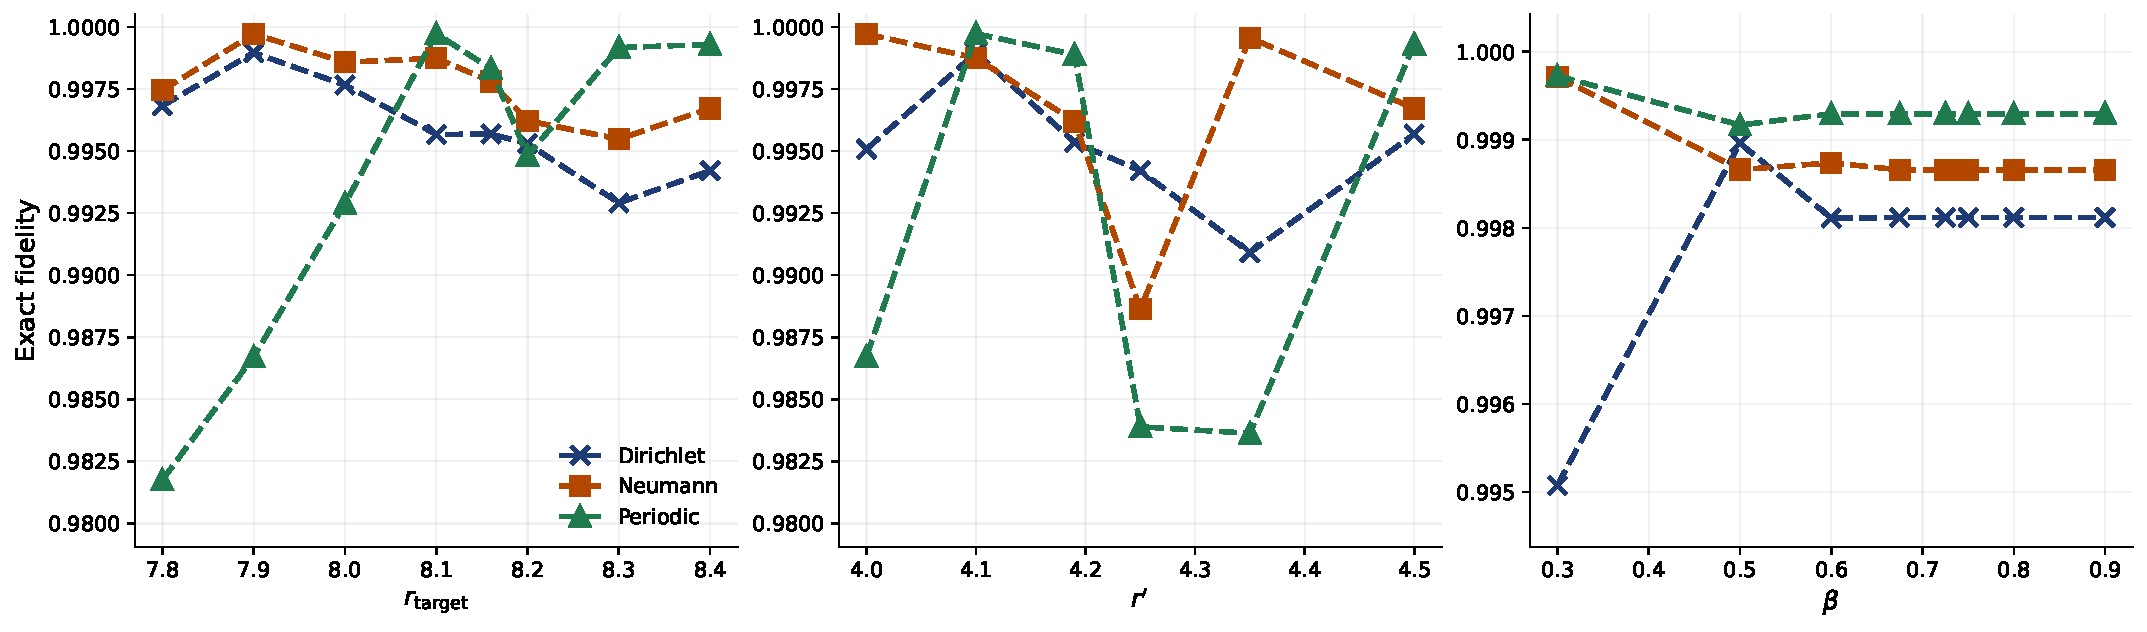
\includegraphics[width=\linewidth]{Pics/section6/section6_sensitivity_exact.pdf}
\caption{Sensitivity of the exact PDE fidelity to the kernel parameters under ideal CV loading. The three panels show, from left to right, variation with $r_{\mathrm{target}}$, $r^\prime$, and $\beta$. For each plotted value on the horizontal axis, the vertical coordinate is the best exact fidelity obtained while the remaining sweep parameters vary over the tested grid.}
\label{fig:clean_sensitivity_exact}
\end{figure}

\begin{table}[h]
\centering
\caption{Parameter choices from the ideal-loading sweep, together with the corresponding fidelities $F_{\mathrm{exact}}$ and $F_{\mathrm{trunc}}$. Here $F_{\mathrm{exact}}$ is measured against the discretized heat-equation solution vector and $F_{\mathrm{trunc}}$ against the finite-Fock CV reference.}
\label{tab:clean_oracle_baseline}
\begin{tabular}{lccccccc}
\toprule
Boundary & $r_{\mathrm{target}}$ & $r^\prime$ & $\beta$ & $n_{\mathrm{coeff}}$ & $F_{\mathrm{exact}}$ & $F_{\mathrm{trunc}}$ & $p_{\mathrm{post}}$ \\
\midrule
Dirichlet & 7.9 & 4.1 & 0.5 & 48 & 0.998961 & 0.999992 & 0.06279 \\
Neumann & 7.9 & 4.0 & 0.3 & 48 & 0.999716 & 0.999984 & 0.05616 \\
Periodic & 8.1 & 4.1 & 0.3 & 48 & 0.999725 & 1.000000 & 0.04842 \\
\bottomrule
\end{tabular}
\end{table}

\subsection{Empirical relation to the theoretical bounds}

Theorem~\ref{thm: state-prep} is asymptotic and contains unspecified constants $\mathcal K$ and $\mathcal M$, which collect the prefactors in the truncation and squeezing estimates. The experiments therefore test qualitative consistency rather than calibrated numerical tightness. Across the ideal-loading parameter study, increasing the oscillator coefficient cutoff from $n_{\mathrm{coeff}}=24$ to $48$ improves the best exact fidelity in all three cases: Dirichlet from $0.9956816$ to $0.9989611$, Neumann from $0.9995599$ to $0.9997155$, and periodic from $0.9992957$ to $0.9997249$. This trend is consistent with Theorem~\ref{thm: state-prep}, which predicts improved approximation as the truncated oscillator resources increase. The same data place the optimum in a large-squeezing regime, with both $r_{\mathrm{target}}$ and $r^\prime$ near $4$ to $8$, again in qualitative agreement with the squeezing dependence of the theorem.

For the hybrid evolution, Eq.~\eqref{eq:heat-trotter-error} predicts first-order scaling in the number of product-formula steps. Using the Dirichlet data and comparing against the truncated CV reference rather than the exact PDE solution, the best observed relative errors are $3.0835\times 10^{-3}$ at $n_{\mathrm{trotter}}=8$, $1.5428\times 10^{-3}$ at $n_{\mathrm{trotter}}=16$, and $7.7171\times 10^{-4}$ at $n_{\mathrm{trotter}}=32$. These values follow a normalized $C/n$ guide line closely, providing a representative empirical check of the expected first-order behavior. This quantitative tightness check is available only for the low-to-moderate Dirichlet sweep region, rather than for the highest-fidelity operating points or uniformly across all three boundary conditions.


\subsection{End-to-end fidelity and state-preparation effects}

Table~\ref{tab:clean_snap_comparison} compares Givens synthesis and SNAP$+$D preparation at the parameter values listed in Table~\ref{tab:clean_oracle_baseline}. The Dirichlet and Neumann SNAP$+$D rows use the best depths identified by the state-preparation study at those kernel points, while the periodic row uses the depth-$6$ optimum at the corresponding periodic kernel point.

The data show that the optimized SNAP$+$D circuits largely close the gap to the ideal baseline for Dirichlet and Neumann. The strongest case is Neumann, where the difference relative to the Givens baseline is only $2.32\times 10^{-4}$. Dirichlet also attains $F_{\mathrm{snap}}=0.993048$, with a remaining difference of $5.91\times 10^{-3}$. The periodic case is less accurate, with a difference of $2.01\times 10^{-2}$.

\begin{table}[t]
\centering
\caption{Givens and SNAP$+$D fidelity comparison at the parameter values in Table~\ref{tab:clean_oracle_baseline}. The Dirichlet and Neumann SNAP$+$D rows use the best depths identified by the state-preparation study at those kernel points, while the periodic row is the depth-$6$ optimum at the corresponding periodic kernel point.}
\label{tab:clean_snap_comparison}
\begin{tabular}{lcccr}
\toprule
Boundary & $F_{\mathrm{givens}}$ & $F_{\mathrm{snap}}$ & $F_{\mathrm{oracle}}$ & Depth \\
\midrule
Dirichlet & 0.998961 & 0.993048 & 0.986509 & 30 \\
Neumann & 0.999716 & 0.999484 & 0.996381 & 30 \\
Periodic & 0.999725 & 0.979594 & 0.800346 & 6 \\
\bottomrule
\end{tabular}
\end{table}

\subsection{Physical interpretation and resource costs}

The high-fidelity oracle-baseline points occur at large values of $r_{\mathrm{target}}$ and $r^\prime$. In the CV-DV LCHS construction, the ancillary oscillator enters through the qumode sandwich $\langle \phi | e^{-it(\hat{x}\otimes L + I\otimes H)} | \psi \rangle$, so these high-squeezing values indicate that the CV resource state must realize a sufficiently broad quadrature-space kernel profile over the relevant spectral window of $A$. The corresponding gain in exact PDE fidelity is accompanied by a smaller postselection probability. At the same time, $F_{\mathrm{trunc}}$ remains essentially unity, showing that once the oscillator seed state is fixed, the hybrid evolution tracks the finite-Fock target very accurately.

The distinction among $F_{\mathrm{oracle}}$, $F_{\mathrm{snap}}$, and $F_{\mathrm{trunc}}$ is physically informative. The quantity $F_{\mathrm{oracle}}$ measures only how accurately SNAP$+$D reproduces the target oscillator seed. The quantity $F_{\mathrm{snap}}$ measures the final PDE solution fidelity, and $F_{\mathrm{trunc}}$ measures agreement with the exact finite-Fock evolution generated by the prepared seed itself. Consequently, $F_{\mathrm{trunc}}\approx 1$ together with a smaller $F_{\mathrm{oracle}}$ shows that the hybrid evolution is accurate once the prepared state is fixed, so the remaining discrepancy is attributable to state preparation rather than to the subsequent CV-DV dynamics. This pattern is visible in the data. For Dirichlet and Neumann, the SNAP$+$D ansatz reaches near-oracle accuracy, with $F_{\mathrm{oracle}}=0.986509$ and $0.996381$ and corresponding end-to-end fidelities $F_{\mathrm{snap}}=0.993048$ and $0.999484$. In the periodic case, by contrast, the circuit still follows the exact truncated map essentially perfectly, but the prepared seed remains the limiting factor, with $F_{\mathrm{oracle}}=0.800346$.

Givens synthesis furnishes an analytic exact-synthesis baseline together with JC-pulse and qubit-rotation counts. In all three boundary conditions, Givens matches the injection fidelity to numerical precision while reporting 47 JC pulses and 47 qubit rotations.

\begin{table}[t]
\centering
{\small
\caption{Representative resource counts for the SNAP$+$D circuits in Table~\ref{tab:clean_snap_comparison} and for the analytic Givens baseline.}
\label{tab:clean_resource_counts}
\begin{tabular}{lcccccc}
\toprule
Boundary & SNAP depth & Circuit depth & Circuit size & Optimizer iters & Givens JC pulses & Givens qubit rotations \\
\midrule
Dirichlet & 30 & 2971 & 3673 & 82 & 47 & 47 \\
Neumann & 30 & 3271 & 3973 & 91 & 47 & 47 \\
Periodic & 6 & 1095 & 1397 & 357 & 47 & 47 \\
\bottomrule
\end{tabular}}
\end{table}

\subsection{Comparison with DV LCHS}

For a discrete-variable LCHS baseline, the first resource question is the size of the quadrature discretization itself. For the homogeneous heat equation considered here, $H=0$ and $L=A^{(\mathrm{bc})}$, so the standard DV LCHS quadrature formulas of Refs.~\cite{LCHS1,LCHS2} give
\[
h_1=\frac{1}{eT\|L\|_2},\qquad
K=\eta\left\lceil \frac{(\log(1/\epsilon))^{1/\beta}}{h_1}\right\rceil h_1,
\]
\[
Q=
\left\lceil
\frac{1}{\log 4}
\log\!\left(
\frac{8}{3C_\beta}\frac{K}{\epsilon}
\right)
\right\rceil,
\qquad
C_\beta = 2\pi e^{-2^\beta},
\]
\[
M_{\mathrm{DV}} = 2\left\lfloor \frac{K}{h_1}\right\rfloor Q,
\qquad
m_c = \left\lceil \log_2 M_{\mathrm{DV}}\right\rceil .
\]
Here $h_1$ is the quadrature step size, $K$ is the truncation half-width of the $k$ interval, $Q$ is the Gauss--Legendre order on each subinterval, $M_{\mathrm{DV}}$ is the resulting number of LCU terms, and $m_c$ is the corresponding control-register width. In Table~\ref{tab:dv_resource_compare} we use $\eta=1$, $\epsilon=0.1$, and a common high-fidelity DV kernel exponent $\beta=0.8$ for all three boundary conditions.

\begin{table}[t]
\centering
{\small
\caption{DV LCHS quadrature parameters for the three heat-equation benchmarks at $\beta=0.8$ and $\epsilon=0.1$.}
\label{tab:dv_resource_compare}
\begin{tabular}{lcccccc}
\toprule
Boundary & $h_1$ & $K$ & $Q$ & $M_{\mathrm{DV}}$ & $m_c$ & $\|c\|_1$ \\
\midrule
Dirichlet & 0.10168 & 2.84702 & 4 & 224 & 8 & 1.0734 \\
Neumann & 0.10775 & 2.90923 & 4 & 216 & 8 & 1.0831 \\
Periodic & 0.09197 & 2.85107 & 4 & 248 & 8 & 1.0740 \\
\bottomrule
\end{tabular}}
\end{table}

This comparison isolates the discretization burden of the DV LCHS quadrature itself. With the present CV truncation $n_{\mathrm{coeff}}=48$, the corresponding DV quadrature term counts are larger by factors of approximately $4.67$, $4.50$, and $5.17$ for Dirichlet, Neumann, and periodic boundary conditions, respectively.

A second comparison concerns circuit realization. On the DV side, the ancilla amplitude vector may be represented as a matrix product state (MPS), i.e.\ a tensor-network factorization into low-rank local tensors along the control register. When the kernel amplitudes admit such compression, the ancilla preparation circuit can be synthesized from the MPS with substantially fewer gates than a generic amplitude-loading routine. For the same Dirichlet benchmark, we therefore consider a DV circuit built from an MPS-compressed ancilla state with $\beta=0.8$. The ancilla preparation and unpreparation are applied once, while only the controlled LCHS evolution block is repeated:
\[
\langle 0_{\mathrm{anc}}|
U_{\mathrm{prep}}^\dagger
\bigl[U_{\mathrm{ctrl}}(T/r)\bigr]^r
U_{\mathrm{prep}}
|0_{\mathrm{anc}}\rangle,
\qquad r=100,
\qquad T=1.
\]
For this Dirichlet instance, the ancilla preparation block contains $130$ single-qubit $u$ gates and $48$ CNOTs, while one controlled-evolution slice contains $38$ CNOTs, $36$ $rz$ gates, $13$ phase gates, $9$ controlled-$rz$ gates, and $4$ Hadamards. The full 100-step DV circuit has depth $9227$ and operator counts
\[
260\,u + 3896\,cx + 3600\,rz + 1300\,p + 900\,crz + 400\,h + x.
\]
By comparison, the Dirichlet SNAP$+$D circuit in Table~\ref{tab:clean_resource_counts} has depth $2971$. Thus, although the DV construction benefits from MPS compression in the ancilla preparation stage, the overall qubit circuit remains deeper for this benchmark.

\begin{table}[t]
\centering
{\small
\caption{Operator counts for the Dirichlet DV LCHS circuit with an MPS-compressed ancilla state and $r=100$ repeated controlled-evolution slices.}
\label{tab:dv_circuit_compare}
\begin{tabular}{lcc}
\toprule
Block & Depth & Operator counts \\
\midrule
Ancilla PREP & 71 & $130\,u + 48\,cx$ \\
One controlled-evolution slice & 91 & $38\,cx + 36\,rz + 13\,p + 9\,crz + 4\,h$ \\
Full 100-step circuit & 9227 & $260\,u + 3896\,cx + 3600\,rz + 1300\,p + 900\,crz + 400\,h + x$ \\
\bottomrule
\end{tabular}}
\end{table}

% \begin{figure}[t]
% \centering
% \[
% \Qcircuit @C=0.72em @R=0.72em {
% \lstick{\ket{0}_{\mathrm{osc}}} &
% \gate{\mathrm{SNAP}(\boldsymbol{\theta}^{(1)})} &
% \gate{D(\alpha_1)} &
% \push{\cdots} &
% \gate{\mathrm{SNAP}(\boldsymbol{\theta}^{(6)})} &
% \gate{D(\alpha_6)} &
% \gate{S(-r^\prime)} &
% \multigate{2}{\left(\mathcal{U}_{II}\,\mathcal{U}_{IX}\,\mathcal{U}_{XX}\,\mathcal{U}_{YY}\,\mathcal{U}_{ZZ}\right)^{100}} &
% \gate{S(r_{\mathrm{target}})} &
% \meter &
% \qw \\
% \lstick{\ket{q_0}} &
% \qw & \qw & \push{\cdots} & \qw & \qw & \multigate{1}{\mathrm{Init}(\ket{u_0})} &
% \ghost{\left(\mathcal{U}_{II}\,\mathcal{U}_{IX}\,\mathcal{U}_{XX}\,\mathcal{U}_{YY}\,\mathcal{U}_{ZZ}\right)^{100}} &
% \qw & \qw & \qw \\
% \lstick{\ket{q_1}} &
% \qw & \qw & \push{\cdots} & \qw & \qw & \qw &
% \ghost{\mathrm{Init}(\ket{u_0})} &
% \ghost{\left(\mathcal{U}_{II}\,\mathcal{U}_{IX}\,\mathcal{U}_{XX}\,\mathcal{U}_{YY}\,\mathcal{U}_{ZZ}\right)^{100}} &
% \qw & \qw & \qw
% }
% \]
% \caption{Representative executed SNAP$+$D circuit for the best practical Neumann run. The Trotter block is implemented in the clean backend as the ordered product 
% \label{fig:circ-snapd}
% \end{figure}



% \begin{figure}[t]
% \centering
% \[
% \Qcircuit @C=0.85em @R=0.80em {
% \lstick{\ket{0}_{\mathrm{osc}}} &
% \multigate{1}{G_{0,1}(\theta_0,\phi_0)} &
% \multigate{1}{G_{1,2}(\theta_1,\phi_1)} &
% \push{\cdots} &
% \multigate{1}{G_{n_{\mathrm{act}}-2,n_{\mathrm{act}}-1}(\theta,\phi)} &
% \qw \\
% \lstick{\ket{0}_{\mathrm{anc}}} &
% \ghost{G_{0,1}(\theta_0,\phi_0)} &
% \ghost{G_{1,2}(\theta_1,\phi_1)} &
% \push{\cdots} &
% \ghost{G_{n_{\mathrm{act}}-2,n_{\mathrm{act}}-1}(\theta,\phi)} &
% \qw
% }
% \]
% \caption{Conceptual Givens synthesis schematic. This diagram is analytic rather than an executed backend circuit in the current clean stack.}
% \label{fig:circ-givens}
% \end{figure}
